\selectlanguage{Brazilian}

\chapter{REVISÃO BIBLIOGRÁFICA}\label{cap2}

A mão foi a principal ferramenta de transformação do meio ambiente do ser humano durante centenas de anos, ela é o principal meio de interação com o ambiente. Pode-se associar o uso das mãos, juntamente com aumento do tamanho cerebral, ao desenvolvimento dos seres humanos em relação ao seus ancestrais. Logo faz sentido projetar manipuladores robóticos quando se pensa na evolução da tecnologia. A ideia é criar membros robóticos que sejam capazes de lidar com o ambiente criado pelas mãos humanas, sem necessariamente executar as mesmas tarefas de pegar e manipular que os humanos são capazes. Com essas habilidades podemos esperar que essas novas ferramentas sejam capazes de performar em ambientes médicos e domésticos \cite{gustus2012human}.
% A modelagem dos componentes da mão (ossos e músculos), assim como do antebraço, são necessários para se prever os eventos físicos de ações desejadas pelo ser humano. Estas podem ser encontradas em diversas áreas como reabilitação de pacientes, manipulação de braços robóticos, biomecânica do esporte e geração de próteses biônicas.

A compreensão das propriedades do movimento, do fluxo necessário para que se ocorra uma ação física humana, é importante quando se quer projetar uma prótese, órtese, ou uma estimulação neuromuscular funcional com o intuito de reaver funções motoras perdidas, este caso se aplica aos engenheiros. E também é importante quando se quer interpretar eventos cinéticos do ser a fim de entender melhor a coordenação do corpo, este caso se aplica aos cientistas \cite{zajac1989muscle}.
% O estudo do monitoramento das mãos começou no período que sucedeu a 2ª Guerra Mundial, com o intuito de desenvolver sistemas de mestre-escravo para manipular os braços \cite{sturman1994survey}.

\section{Tecnologias de Miografia}\label{cap2:sub2}

Desde os anos de 1960 o conceito de criar uma interface para comunicação eletrônica com o sistema nervoso humano é amplamente estudado. Trabalhos mostram que próteses enervadas aumentarão e melhorarão as capacidades do ser humano \cite{gasson2005invasive}.  As técnicas de miografia se baseiam em um pilar que é a comunicação, e infelizmente, para os membros biônicos atuais este é o elo mais fraco da relação usuário-dispositivo. Hoje pode-se dividir as pessoas que utilizam desta tecnologia em dois grupos distintos: (i) aquelas que precisam de uma interface que obtém os sinais cognitivos e os decifra para construir o movimento e (ii) aquelas que ainda possuem algum resíduo  de controle sobre funções motoras relevantes \cite{craelius2002}. 

Em ambos os casos são utilizadas tecnologias de miografia, invasivas e não-invasivas, com o intuito de criar esta interface entre o usuário e o membro prostético. No primeiro grupo (i) é necessário um tipo de miografia invasiva, que obtém os sinais cognitivos vindos do cérebro, os decifra e converte em ações em algum membro biônico. Já para o segundo grupo (ii) técnicas de miografia não invasiva são suficientes para controlar os membros biônicos já que as intenções musculares podem ser obtidas através, por exemplo, de sensores de superfície.

% Próteses encontraram mais obstáculos a partir do momento que as amputações perdiam mais músculos, um caso mais complexo variante do grupo (i), por exemplo uma amputação completa do braço, a partir dai, o procedimento para aplicação de tecnologias de controle de próteses foi transportar músculos de outras partes do corpo para a área amputada, como por exemplo do peito do paciente, e de reconstrução dos nervos dessa área cirurgicamente, com isso, os sinais poderiam chegar novamente nos sensores das próteses, essa tática é denominada TMR (\textit{Targeted Muscle Reinnervation}) \cite{lipschutz2006shoulder}.

\subsection{Miografia de Profundidade}\label{cap2:sub2.1}

H. Piper é considerado o primeiro a estudar os sinais de eletromiografia em 1912 na Alemanha utilizando um galvanômetro de corda \cite{merletti2004electromyography}. A miografia está fundamentada no fenômeno conhecido como potencial de ação. Este impulso elétrico gerado pelo corpo humano causa distúrbios na fibra muscular como o encurtamento ou deslizamento de suas estruturas no acoplamento eletromecânico \cite{rodriguez2000eletromiografia}. A eletromiografia de profundidade (EMG) é uma técnica invasiva, onde os eletrodos são colocados no interior do músuculo fazendo contato com as fibras musculares. Os eletrodos são responsáveis por captar diretamente os sinais elétricos produzidos pelo potencial de ação ocorrido nas fibras musculares e transmitir esse sinal para que seja analisado \cite{merletti2004electromyography}. 

A grande desvantagem deste tipo de técnica é que ela é altamente invasiva, é necessário que um instrumento penetre na pele do objeto de estudo para que os sinais possam ser coletados, porém a EMG de profundidade consegue detectar informações muito localizadas tanto para músculos superficiais quanto para músculos mais profundos \cite{merletti2004electromyography}. Um exemplo da vantagem da EMG pode ser notada na figura \ref{Merletti2004_EMG}, no caso foi usado eletrodo em forma de agulha concêntrica, e é perceptível notar como a técnica é precisa a ponto de receber com maior amplitude os potenciais de ação das fibras específicas requisitadas para o estudo realizado.
 
\begin{figure}[H]
\centering
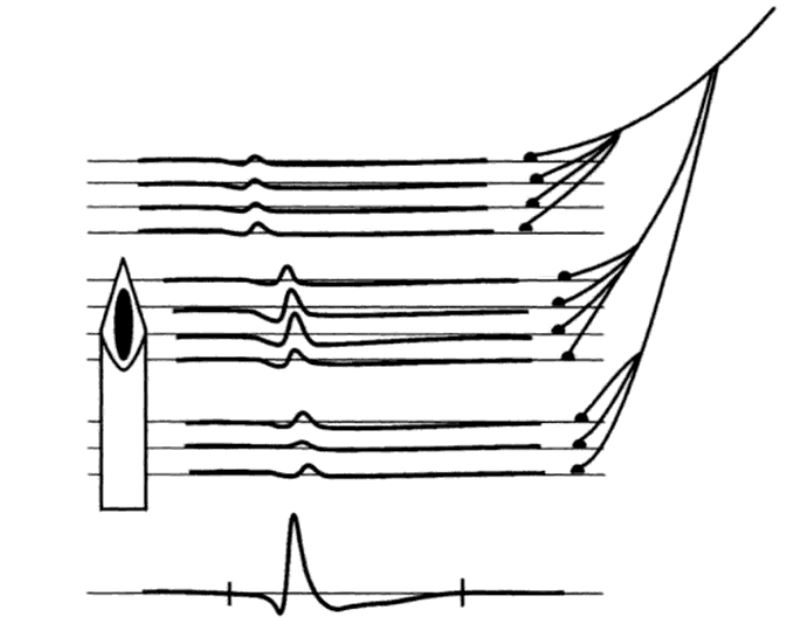
\includegraphics[width = 0.8\textwidth]{img/Merletti2004_EMG.JPG}
\caption[Eletrodo em Forma de Agulha Para Eletromiografia de Profundidade]{Unidade motora do potencial de ação detectada por um eletrodo em forma de agulha concênctrica. Os potenciais de ação das fibras musculares mais próximas são detectados com maior amplitude que os potenciais das fibras mais distantes. A chegada dos potenciais de ação individuais de cada fibra no eletrodo não é perfeitamente síncrono \cite{merletti2004electromyography}.}
\label{Merletti2004_EMG}
\end{figure}

\subsection{Interface Cérebro-Computador}\label{cap2:sub2.2}

As BCI (Brain-Computer Interface), como são conhecidas as interfaces cérebro-computador, são interfaces que interagem diretamente com o sistema nervoso transformando atividade metabólica cerebral em sinais de controle para dispositivos e aplicações \cite{scherer2007self}, neste caso seriam as intenções de ação de um ser humano. Estes sinais elétricos, conhecidos como sinais eletroencefalográficos, são coletados no escalpo humano e representam flutuações do potencial elétrico correspondentes a variações nas camadas mais externas do córtex cerebral abaixo do escalpo \cite{vidal1973toward}. Assim como a técnica citada em \ref{cap2:sub2.1}, a maior parte das técnicas utilizadas pelas BCI consistem de um estilo de miografia invasiva pois os sinais elétricos são adquiridos diretamente do cérebro do usuário através do escalpo, como foi feito no estudo de \cite{hochberg2012reach}, em que os objetos de estudo deveriam movimentar um braço robótico com um BCI implantado em suas cabeças. 

Dentre as dificuldades que esta técnica enfrenta estão as questões éticas. Para os métodos invasivos de obtenção de dados os estudiosos dizem que esse tipo de tecnologia pode possivelmente levar a perdas neurais significantes e risco de infecção, ainda mais se forem feitas conexões de longo período. E mesmo para os métodos não invasivos, como o electroencefalográfico (EEG) \cite{daly2009feasibility}, para BCI existem questionamentos quanto a invasão de privacidade, já que se torna possível o uso da tecnologia para obtenção de dados sigilosos do usuário sem a sua aprovação \cite{wolpaw2006bci}. Por outro lado o uso da BCI é extenso quando se trata da gama de usuários que podem utilizá-la. Os usuários que desfrutam da BCI podem ser divididos em três grupos, (i) aqueles que não possuem nenhum tipo de controle neuromuscular (incluindo movimento dos olhos), (ii) os que possuem uma capacidade limitada de controle neuromuscular e (iii) os que ainda possuem uma quantidade considerável de controle neuromuscular (como a fala e  controle da mão). Assim pode-se entender que o uso de BCI pelos usuários está mais ligado a extensão da disfunção corporal que a origem da disfunção \cite{wolpaw2006bci}.

\begin{figure}[H]
\centering
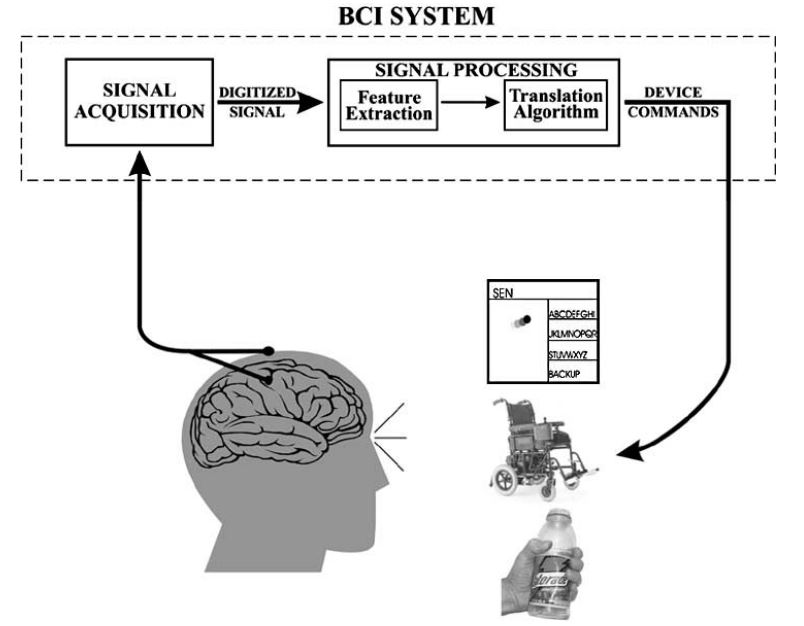
\includegraphics[width = 0.8\textwidth]{img/Schalk2004_BCI.JPG}
\caption[Design Básico de Operação para Qualquer Sistema BCI]{Design básico de operação de qualquer sistema BCI. Sinais que são adiquiridos do cérebro por eletrodos no escalpo, no córtex cerebral ou dentro do cérebro, são processados para extrair aspectos específicos (como amplitudes de potenciais reativos ou ritmos do cortex sensomotor, padrões reativos de neurônios corticais) que refletem a intenção do usuário. Características são traduzidas em comandos que operam um dispositivo (isto é, um simples programa de processamento de palavras, uma cadeira elétrica ou uma prótese neural) \cite{schalk2004bci2000}.}
\label{Schalk2004_BCI}
\end{figure}

\subsection{Eletromiografia de superfície}\label{cap2:sub2.3}

Se um par de eletrodos é colocado na pele de um usuário, sobre o seu músculo, e este é ativado voluntariamente, é possível obter um sinal elétrico entre os eletrodos \cite{merletti2001surface}. Portanto a técnica de eletromiografia de superfície (sEMG) é considerada uma técnica de miografia não invasiva. Desde os anos 1960 a sEMG (\textit{surface electromyography}) é utilizada para controlar manipuladores robóticos em forma de mão com um grau de liberdade já que, como uma técnica não invasiva, dispensa cirurgias ou internação, e mesmo após anos de uma amputação os sinais continuam claros e mais puros que os obtidos diretamente do cérebro, através de métodos não invasivos \cite{castellini2014proceedings}. Apesar de extensamente estudada, a sEMG ainda apresenta limitações no que tange a sua aplicação para membros biônicos como, por exemplo, falta de robustez nas medições, que eram alteradas por eventos fisiológicos dos pacientes, como o suor na pele e a fadiga do músculo \cite{castellini2014proceedings}.

\begin{figure}[H]
\centering
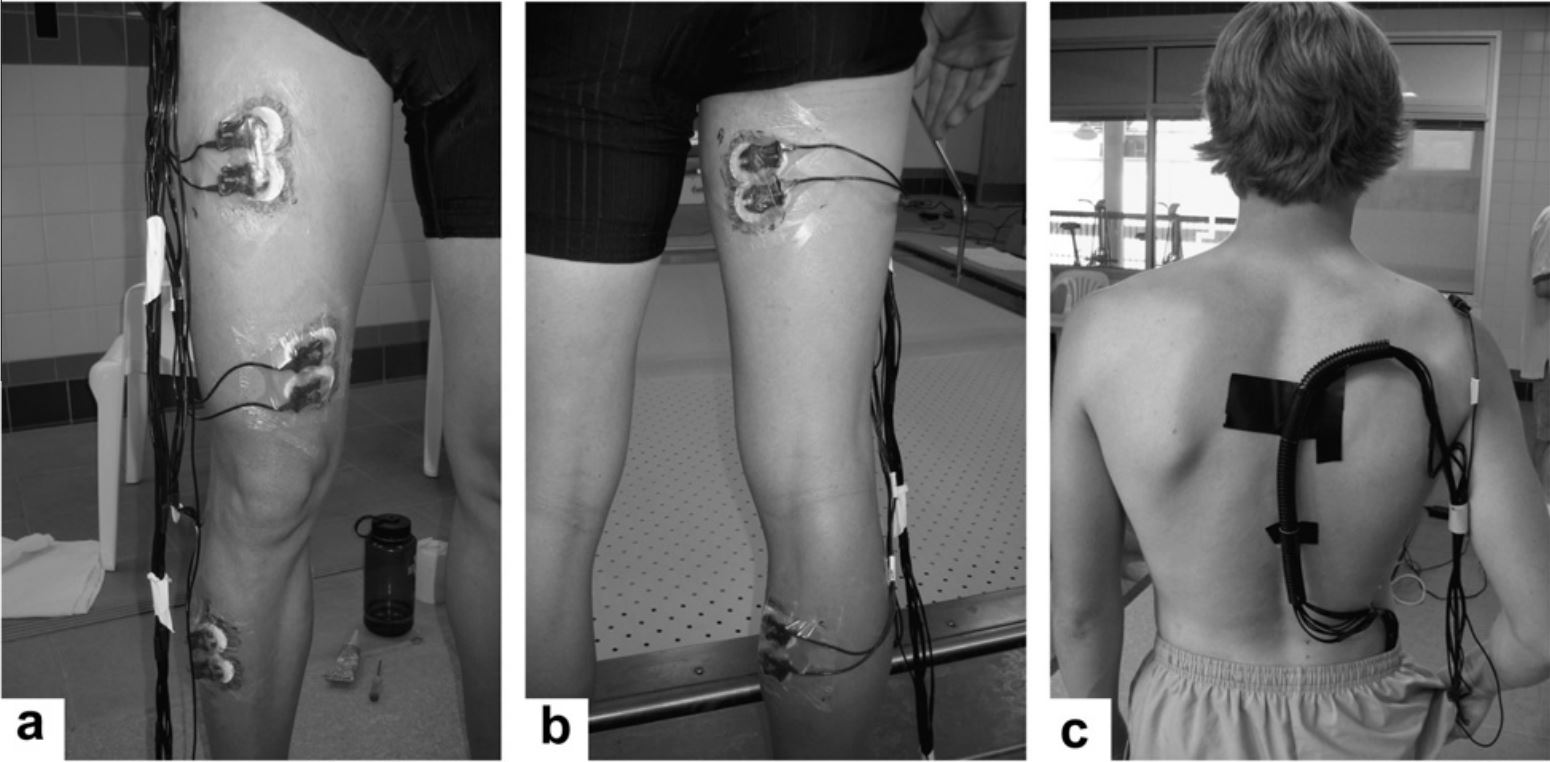
\includegraphics[width = 0.8\textwidth]{img/Silvers2009_sEMG.JPG}
\caption[Montagem Para Testes de Contração Muscular Submerso em Água]{Os fios foram guidaos ao longo da lateral da perna direita (a,b) até a área lombar, onde foram unidos por um tubo plástico, passando pela espinha torácica (c)\cite{silvers2011comparison}.}
\label{Silvers2009_sEMG}
\end{figure}
		

\subsection{Mecanomiografia}\label{cap2:sub2.4}

Com o avanço das técnicas não invasivas surgiu um tipo de tecnologia que remete a observações feitas há mais de trezentos anos, as quais possuiam limitações que não permitiram o seu desenvolvimento tecnológico na época. A tecnologia em questão é a mecanomiografia (MMG), uma técnica que registra as vibrações ou sons produzidos pelo músculo esquelético ao se contrair \cite{vaz1999mecanomiografia} \cite{shinohara1997mechanomyography}.

A MMG se baseia no fato de que as vibrações do músculo ao se contrair são causadas pela contração tetânica incompleta das unidades motoras, portanto é uma técnica não-invasiva, e algumas aplicações deste tipo de miografia incluem o estudo do padrão da fadiga muscular, controle motor, propriedades musculares, frequência da ressonância do músculo e estimativa da força do músculo \cite{shin2016fatigue}. Uma das desvantagens mostradas pelas pequisas sobre esta técnica é a relação entre a taxa de disparo de uma unidade motora e a frequência de informações no sinal da MMG \cite{shin2016fatigue}\cite{shinohara2006mechanomyography}, assim como a dificuldade na montagem para alguns procedimentos o que a torna inviável para algumas rotinas clínicas \cite{hemmerling2004phonomyography}. 

A MMG pode ser um método melhor para aquisição de dados pois possui menos impedimentos, erros no sinal adquirido e processamento de sinal que a sEMG \cite{al2014novel}. Como a amplitude do sinal na MMG é relacionada com a produção de força no músculo, então até uma pequena alteração na força já demonstra alteração no sinal adquirido, enquanto pequenas mudanças de força não são refletidas no sinal adquirido da sEMG \cite{sarillee2014non}.

\begin{figure}[H]
\centering
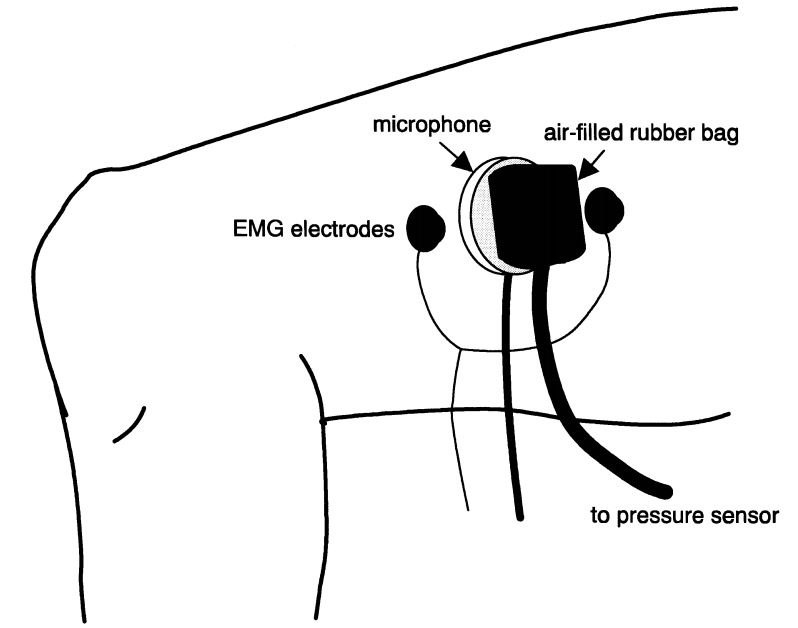
\includegraphics[width = 0.8\textwidth]{img/Shinohara1997_MMG.JPG}
\caption[Diagrama da Montagem Para Medição da EMG, MMG e Pressão]{Diagrama da montagem para a medição da eletromiografia (EMG), a mecanomiografia (MMG), e pressão\cite{shinohara1997mechanomyography}.}
\label{Shinohara1997_MMG}
\end{figure}
 
\subsection{Miografia de Força}\label{cap2:sub2.5}

Tentando melhorar a captação de sinais dos movimentos voluntários, surgem novas técnicas utilizando tecnologias diferentes para superar as barreiras impostas pelos outros métodos já citados. Um novo método que começou a ser desenvolvido recentemente é a miografia de força (FMG). Este método é baseado na medidas dos padrões de resposta mecânica, a força do músculo é medida utilizando um conjunto de sensores de força sobre o músculo para gerar um mapa topográfico de força da atividade muscular e assim decodificar os comandos motores \cite{rasouli2015stable}. Uma aplicação da tecnologia foi estudada em \cite{ravindra2014comparative}, onde foram testadas 3 tecnologias de miografia não invasivas, neste estudo foram analisadas as capacidades de se controlar uma mão prostética de múltiplos dedos. No estudo de \cite{ravindra2014comparative} pode-se notar que a tecnologia da FMG se sobrepõe a EMG pois ela continua com as leituras estáveis mesmo após algum tempo, que é uma das desvantagens da EMG, a fadiga do músculo.

\begin{figure}[H]
\centering
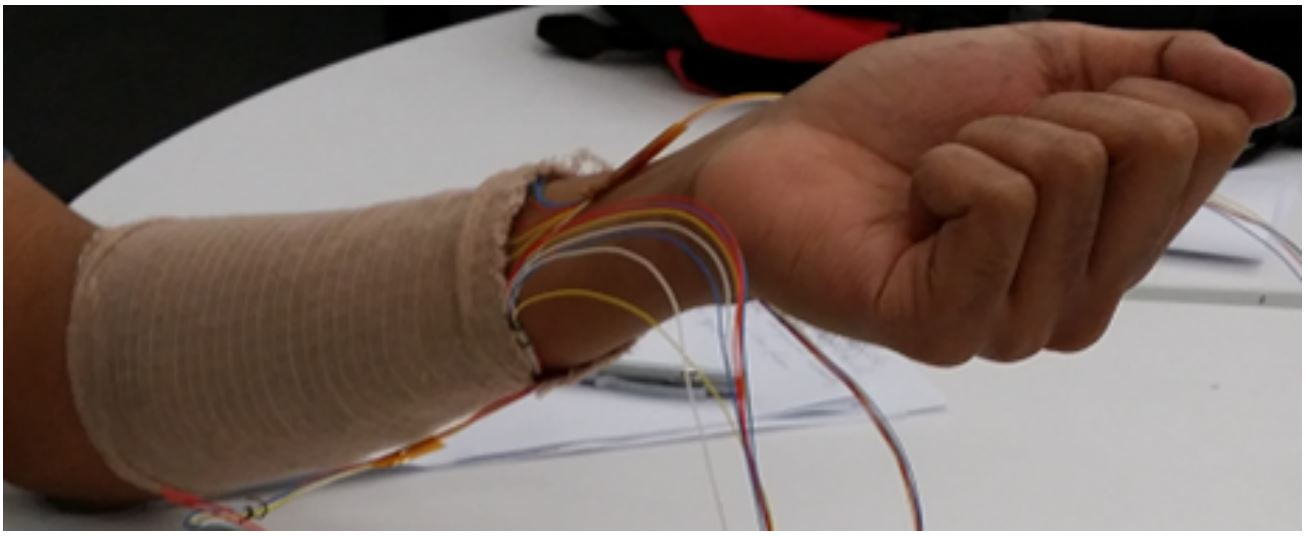
\includegraphics[width = 0.8\textwidth]{img/Rasouli2015_FMG2.JPG}
\caption[Montagem Experimental da FMG]{Montagem experimental de \cite{rasouli2015stable} para obtenção dos sinais de força pela FMG.}
\label{Rasouli2015_FMG}
\end{figure}

\section{Cinemática da Mão}

\subsection{Anatomia da Mão}
\label{anatomia_mao}
A mão humana, como já dito, é uma ferramenta dotada de grande riqueza funcional graças à sua função principal: a preensão. O ser humano é o único capaz de realizar tal ação em um grau de perfeição, e isto se dá ao fato de apresentar um polegar opositor. A mão representa a \textit{"extremidade realizadora"} do membro superior e é altamente articulada \cite{kapandji1971physiology}. 

Para modelar a articulação dos dedos é necessário definir a estrutura cinemática da mão. A mão possui 4 tipos básicos de ossos: metacarpos; falanges próximas; falanges médias; e falanges distais. E possui 4 tipo de juntas básicas: interfalangial distal (DIP); interfalangial próxima (PIP); metacarpofalangial (MP); e interfalangial (IP). A anatomia dos ossos e juntos da mão humana é mostrada na figura \ref{Lee_Kunis_Mao}, na mesma figura os dedos são referenciados como sendo: I - Polegar; II - Indicador; III - Médio; IV - Anelar; e V - Mínimo. As juntas são responsáveis por dar a mão os graus de liberdade (GL), e existem 4 tipos de juntas neste caso: torção, flexão, diretiva e esférica. As juntas de torção e flexão (com um GL) representam a pronação do antebraço e os movimentos de joelho ou ombro, respectivamente. A junta diretiva (com dois GL) permite a flexão em duas direções distintas. A junta esférica (com três GL) permite movimentos diretivos e de torção ao mesmo tempo \cite{lee1995model}. Portanto para os dedos indicador, médio, anelar e mínimo pode ser usada a mesma modelagem cinemática, onde são definidos 4 GL, e não se considera a junta da palma da mão, a qual adicionaria mais um grau de liberdade. E o polegar apresenta 5 GL\cite{lee1995model}.

\begin{figure}[H]
\centering
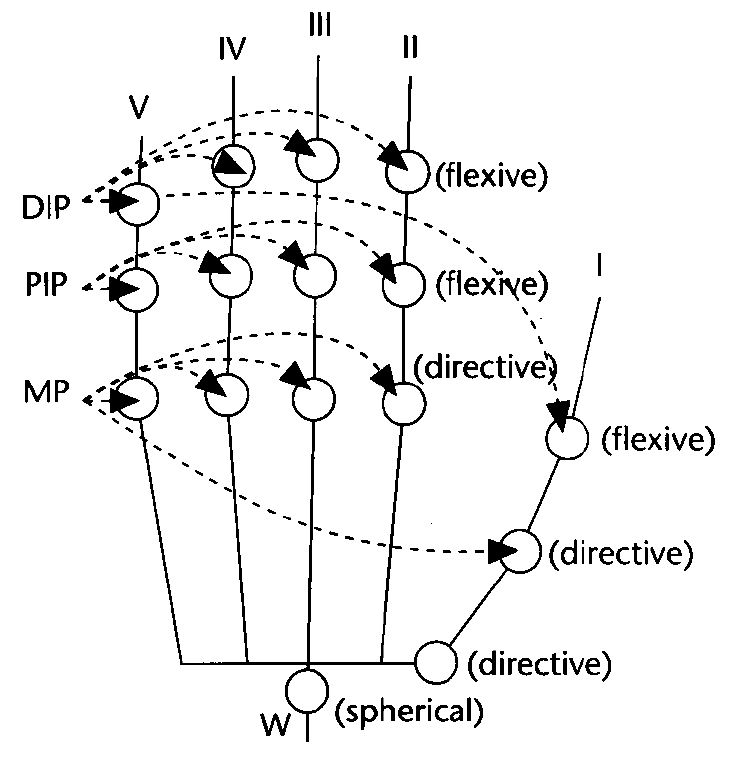
\includegraphics[width = 0.8\textwidth]{img/Lee_Kunis_Mao.JPG}
\caption[O esqueleto da mão observado pelo lado da palma]{Esqueleto da Mão \cite{lee1995model}.}
\label{Lee_Kunis_Mao}
\end{figure}

Existem trabalhos que abordam diferentes modelos para a mão humana.  \cite{bray2005stochastic} propõe um modelo com 26 GL, \cite{kuch1994human} descreve um modelo com 23 GL, \cite{chalfoun2004muscle} e \cite{renault2001dynamic} propõem um modelo com 20 GL, enquanto \cite{du20073d} traz um modelo de 26 GL. No trabalho de \cite{cobos2008efficient} é utilizado um modelo de 24 GL contra dois modelos de 9 e 6 GL, afim de discutir os erros de posição que a diferença de GL proporciona. Os modelos apresentam diferentes GL devido as restrições, impedindo que a mão não possa fazer gestos arbitrários. Por exemplo o dedo mínimo não consegue ser dobrado sem que se dobre o dedo anelar \cite{lin2000modeling}.

Segundo \cite{lin2000modeling} as restrições da mão podem ser divididas em três tipos. Restrições do tipo 1 são referentes aos limites dos movimentos dos dedos como resultado da anatomia da mão. Restrições do tipo 2 são limites impostos nas juntas quando em movimento. Restrições do tipo 3 acontecem devido a performance natural da mão, e ainda não foram amplamente estudadas.

\subsubsection{Restrições do Tipo 1}\label{Tipo 1}
Este tipo de restrição está atrelado aos limites de alcance da movimentação dos dedos como um resultado da anatomia da mão. Neste caso para se impor a restrição é necessário levar em conta que não há forças externas atuando sobre o movimento dos dedos. Portanto podemos determinar restrições como:

\begin{align}
0^\circ < \theta_{MP_F} \leq 90^\circ, \\
0^\circ < \theta_{PIP_F} \leq 110^\circ, \\
0^\circ < \theta_{DIP_F} \leq 90^\circ, \\
-15^\circ < \theta_{MP_{AA}} \leq 15^\circ.
\end{align}

onde o subescrito F se aplica para o movimento de flexão e o subescrito AA o movimento de abdução e adução.

Outra restrição usualmente adotada é relativa aos movimentos de abdução e adução do dedo médio, pois neste são quase inexistentes. Da mesma maneira, a junta metacarpofalangial do polegar não apresenta tais movimentos de abdução e adução.

\begin{align}
\theta_{MP_{AA}} = 0^\circ
\end{align}

Os dedos indicador, médio, anelar e mínimo são considerados manipuladores planares, ou seja, das juntas DIP, PIP e IP de cada dedo se movimentam em apenas um plano, já que as juntas DIP e PIP possuem um grau de liberdade \cite{lin2000modeling}.

\subsubsection{Restrições do Tipo 2}\label{sssec:Tipo2}
Este tipo de restrição se refere aos limites impostos nas juntas durante a movimentação dos dedos. Estas restrições podem em si serem divididas em outras duas subdivisões, uma relativa ao movimento do dedo consigo mesmo e a outra relativa ao movimento de um dedo em relação a outro.

As relações entre dedos é dada entre juntas de dedos adjacentes, como por exemplo quando a junta MP do dedo indicador é dobrada, a junta MP do dedo médio é forçada a se dobrar também \cite{lin2000modeling}.

A relação entre as juntas de um mesmo dedo é frequentemente representada pela restrição em que quando a junta DIP é dobrada, a junta PIP correspondente deve ser dobrada também \cite{lin2000modeling}\cite{lee1995model}. Esta restrição pode ser aproximada de tal forma que:

\begin{align}
\theta_{DIP} = \frac{2}{3} \theta_{PIP}
\end{align}

\subsubsection{Restrições do Tipo 3}\label{Tipo 3}
Segundo \cite{lin2000modeling} estas restrições são impostas pela natureza dos movimentos da mão humana e portanto são mais difíceis de se detectar e quantificar. As restrições do tipo 3 se diferem das restrições do tipo 2 pelo fato de não estarem atreladas as limitações da anatomia da mão humana, mas são um resultado de movimentos naturais. Por exemplo, a maneira mais natural de se fechar a mão é flexionando todos os dedos quase que ao mesmo tempo, ao invés de curvar um dedo de cada vez. Este tipo de restrição não pode ser representado por uma equação já que difere de pessoa para pessoa e ao mesmo tempo é similar para muitos.

\subsection{Propriedades e Modelos dos Músculos}\label{propriedades_musculo}
A partir do modelo cinemático da mão pode-se estabelecer a relação entre o ângulo formado pelas juntas dos dedos e a posição final da ponta dos dedos. Para que o dedo assuma tal posição, de forma direta, se faz necessário determinar como os músculos dos membros superiores, majoritariamente mão e antebraço, funcionam com o objetivo de movimentar o dedo de tal forma que a sua ponta atinja o ponto final.

\subsubsection{Anatomia Muscular}
Os músculos podem ser considerados um conjuntos de fibras igualmente longas, chamadas de células, em paralelo. As fibras do músculo estão orientadas em direção do tendão ou em um ângulo agudo em relação ao tendão, como demonstrado na figura \ref{fibras}, sendo $\alpha$ o ângulo agudo. Este ângulo $\alpha$ representa a orientação das fibras em relação ao eixo de ação do tendão. Pode-se notar que conforme o tendão se estica, $\alpha$ aumenta e assim sendo as fibras contraem em uma direção que não é colinear com a direção em que o tendão estica \cite{zajac1989muscle}.

\begin{figure}[H]
\centering
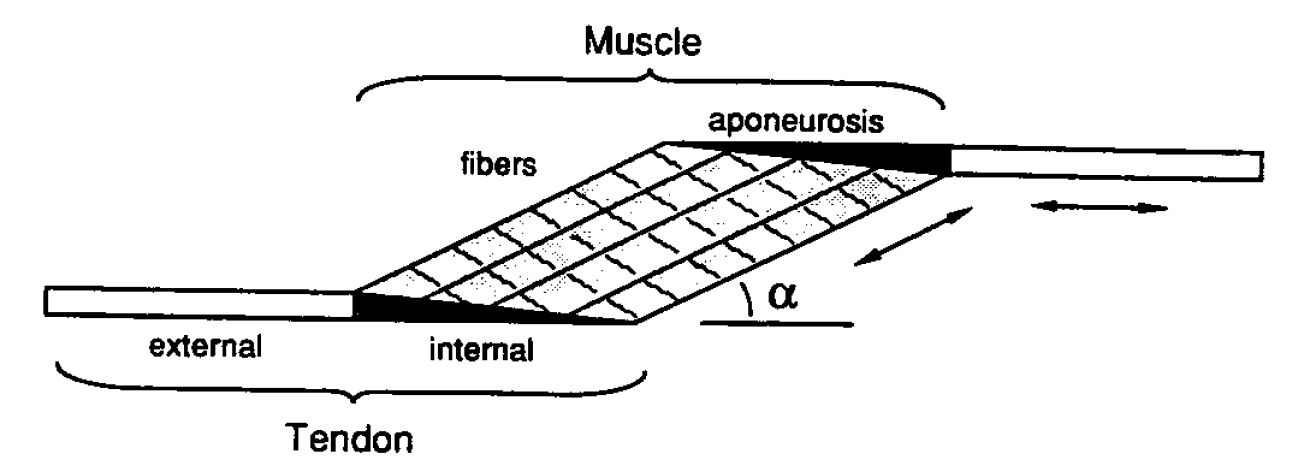
\includegraphics[width = 0.8\textwidth]{img/Zajac1989_FibrasMusculares.JPG}
\caption[Representação das Fibras Musculares]{Relação entre as fibras musculares e o tendão em um músculo penado \cite{zajac1989muscle}}
\label{fibras}
\end{figure}

Uma fibra muscular de tamanho $L_m$ pode ser considerada um conjunto de sarcômeros de mesmo tamanho $L_s$, os quais são estimulados simultaneamente para produzir a força F, demonstrados na figura \ref{sarcomeros}. Os sarcômeros, por sua vez, são constítuidos de filamentos finos (actina) e espessos (miosina) que deslizam entre si para produzir o movimento de contração do músculo.

\begin{figure}[H]
\centering
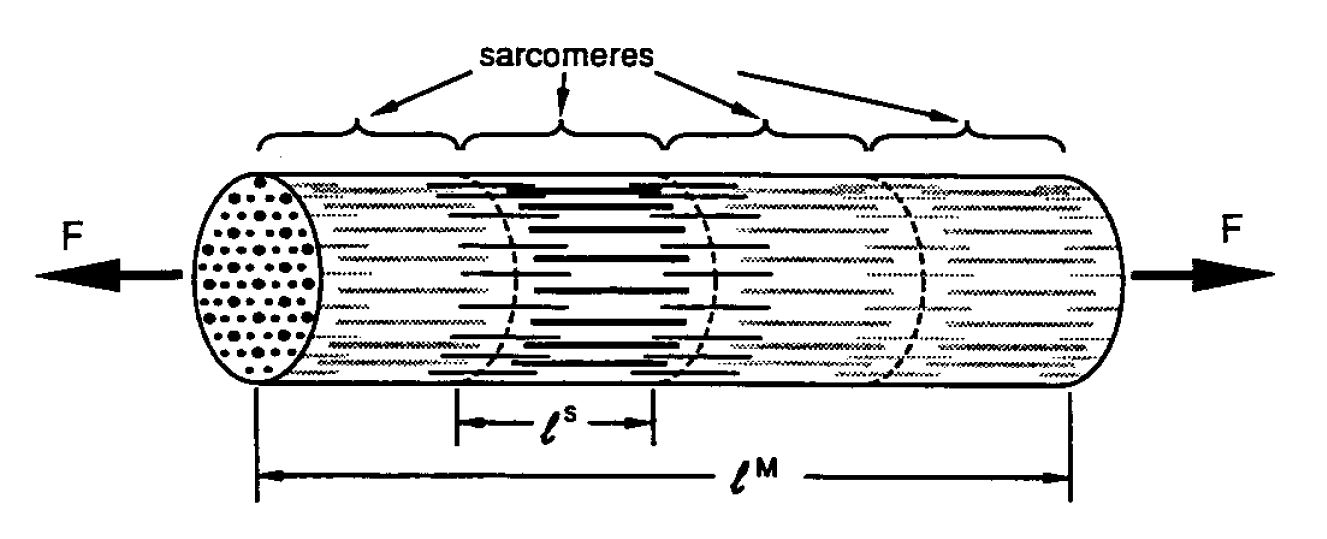
\includegraphics[width = 0.8\textwidth]{img/Zajac1989_Sarcomeros.JPG}
\caption[Representação dos Sarcômeros]{Representação da fibra muscular e a estrutura de sarcômeros \cite{zajac1989muscle}}
\label{sarcomeros}
\end{figure}

Uma unidade motora é definida como um axônio e um conjunto de fibras musculares enervadas por este axônio e seus ramos \cite{burke2011motor}. Um músculo pode ser representado por \textit{n} unidades motoras sendo controladas por \textit{n} axônios originados no sistema nervoso central, cada um deles com o seu controle $u_i(t)$. A força $F^i_m$, originada em uma unidade motora, é proveniente das fibras musculares que agem em conjunto para desenvolvê-la, como é representado na figura \ref{unidademotora}.  Pode-se dizer, então, que a soma das forças $F^i_m$ produzem a força muscular líquida $F_m$.

\begin{figure}[H]
\centering
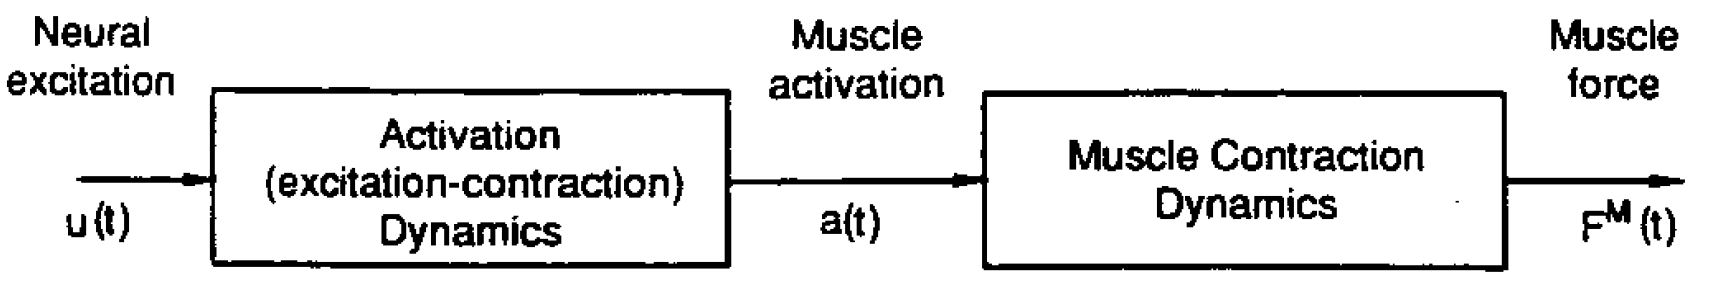
\includegraphics[width = 0.8\textwidth]{img/Zajac1989_UnidadeMotora.JPG}
\caption[Representação da Produção de Força em uma Unidade Motora]{Dinâmimca do tecido muscular\cite{zajac1989muscle}}
\label{unidademotora}
\end{figure}

A dinânimca contracional do músculo pode ser dividida entre: dinâmica de ativação e dinâmica de contração. A dinâmica de ativação diz respeito a transformação de estímulos neurais em ativação dos elementos contráteis. A dinâmica de contração diz respeito a transformação de ativação em força muscular. Existem duas propriedades que discutem a dinâmica de contração: a propriedade de força-comprimento, que diz respeito a capacidade do tecido muscular em gerar força enquanto se alonga, e a propriedade de força-velocidade, que diz respeito a velocidade em que as fibras finas e espessas se deslocam ao realizar a contração e a quantidade de pontes cruzadas no tecido muscular \cite{zajac1989muscle}.

\subsubsection{Modelo de Hill}
O modelo que descreve uma fibra muscular e é amplamente utilizado na literatura é o modelo de Hill, de 1938 \cite{hill1938heat}. Este modelo parte do pressuposto que as propriedades de contração de um tecido muscular podem ser representadas por uma relação de força-comprimento-velocidade (\textit{flv}) 

A versão simplificada deste modelo é baseada em 3 componentes, presentes na figura \ref{hillmodel}: elemento contrátil (CE), representado por um amortecedor, e mostra a relação entre a intensidade e velocidade da força exercida pelo músculo; elemento elástico em série (SE); e elemento elástico em paralelo (PE). Os elementos SE e PE representam a conexão passiva do tecido, incluindo tendão e fibras musculares não ativas \cite{rosen1999performances}

\begin{figure}[H]
\centering
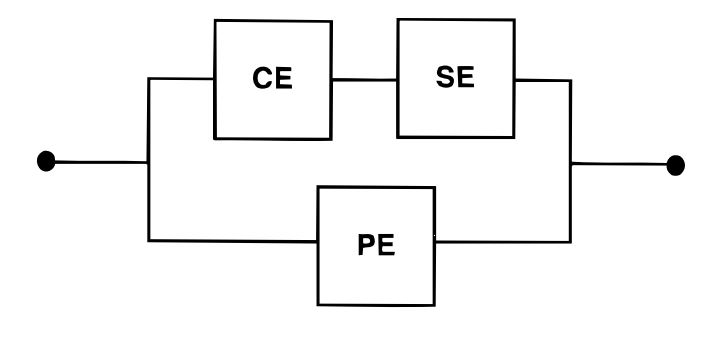
\includegraphics[width = 0.8\textwidth]{img/Rosen1999.JPG}
\caption[Modelo de Hill para uma fibra muscular]{Modelo de Hill para uma fibra muscular. PE = Elemento Elástico Paralelo; CE = Elemento Contrátil; SE = Elemento Elástico em Série \cite{rosen1999performances}.}
\label{hillmodel}
\end{figure}

Mesmo que este modelo seja uma versão simplificada e possua limitações ele é amplamente utilizado devido a facilidade da sua implementação \cite{rosen1999performances}. O modelo de Hill foi aprimorado com o tempo por pesquisadores diferentes, o modelo apresentado no trabalho de \cite{rosen1999performances} tem como base outros trabalhos anteriores como os de Winters (\cite{winters1993effect}, \cite{winters1985task}, \cite{winters1987biomechanical}, \cite{winters1988estimated}). 

Segundo \cite{rosen1999performances} a relação entre força e extensão dos tecidos são definidas pelas seguintes equações:

\begin{align}
F_{SE}=\frac{F_{SEmax}}{e^{SEsh}-1}(e^{SE_{sh}\Delta L_{SE}/\Delta L_{SE_{max}}}-1) \label{forcaSE} \\
F_{SE}=\frac{F_{PEmax}}{e^{PEsh}-1}(e^{PE_{sh}\Delta L_{PE}/\Delta L_{PE_{max}}}-1) \label{forcaPE}
\end{align}

Estas relações representam o comportamento do músculo no esqueleto, como a força exercida pelos componentes se relaciona ao comprimento dos componentes. $F_{SE}, \Delta L_{SE}$ e $F_{PE},\Delta L_{PE}$ são, respectivamente, a força e a extensão de cada componente, e o subescrito \textit{max} denota os valores máximos para o correspondente. $SE_{sh}$ e $PE_{sh}$ são parâmetros em função da forma ("\textit{shape}").

O componente elástico (CE) representa as fibras ativas do músculo e existem duas relações para definí-lo: a relação força-comprimento e a relação força-velocidade. \cite{rosen1999performances} representa a força total gerada por CE como:

\begin{align}
F_{CE} = f_{FV}(V_{CE}) \cdot f_{FL}(L_{CE}) \cdot F_{max} \cdot U \label{forcaCE}
\end{align}

Onde $F_{CE}$ é a força no componente CE, $f_{FV}$ e $f_{FL}$ são funções adimensionais para força-velocidade e força-comprimento, respectivamente. $F_{max}$ é a força máxima em CE, $V_{CE}$ e $L_{CE}$ são, respectivamente, a velocidade de deslocamento e o próprio comprimento de CE, $U$ é o nível normalizado de ativação do componente. O nível de ativação do músculo tem o objetivo de diferenciar movimentos suaves de movimentos fortes. As funções $f_{fv}$ e $f_{FL}$ são descritas em \ref{funcveloc} e \ref{funcdesloc}

\begin{align}
f_{FV} = \frac{0,1433}{0,01074+ e^{-1,409sinh(3,2V_{CE}/V_{max}+1,6)}} \label{funcveloc} \\
f_{Fl} = e^{(-0,5((L_{CE}/L_0-1,05)/0,19)^2} \label{funcdesloc}
\end{align}


Onde $L_{CE}$ e $L_0$ são o comprimento do músculo e o comprimento do músculo relaxado, respectivamente. $V_{max}$ e $V_{0}$ são a velocidade máxima do músculo e a velocidade específica para a ativação do músculo no momento do movimento desejado, respectivamente.

Com as equações de \ref{forcaSE} até \ref{funcdesloc} é possível prever a força que será realizada pelo músculo com o uso apenas de dados anatômicos do ser humano em questão, o que torna o estudo escalável.